\subsection{Uczenie nadzorowane i nienadzorowane - charakterystyka, metody i zastosowania}

\begin{figure}[H]
	\centering
	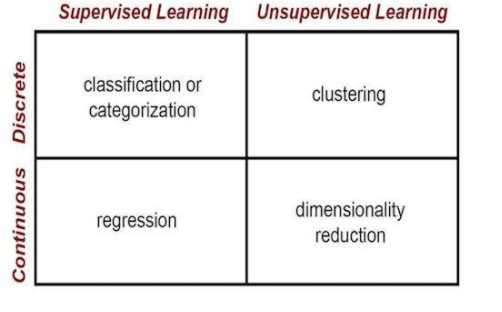
\includegraphics[width=0.5\linewidth]{S1.png}
	\caption{TLDR Uczenia Maszynowego}
\end{figure}

\subsubsection{Charakterystyka}

\centerline{\textbf{Uczenie nadzorowane}}

Jeżeli zbiór danych zawiera pary składające się z: \textbf{wejściowego obiektu uczącego} (np. wektor) oraz \textbf{pożądaną odpowiedź} (np. klasę), to mamy do czynienia z \textbf{uczeniem nadzorowanym}. \\

Załóżmy, że znamy wartości pomiarów ($X$) i oraz klasyfikację/ocenę pomiarów ($Y$). Do klasyfikacji możemy posłużyć się mapowaniem: $Y=f(X)$. Celem uczenia nadzorowanego jest wyznaczenie funkcji $f$ potrafiącej wyznaczyć klasyfikację $Y$ dla dowolnych pomiarów $X$ spoza posiadanego zbioru uczącego. \\

Proces nauki polega na iteracyjnym przetwarzaniu próbek treningowych. Dla każdej próbki wyznaczany jest błąd predykcji, definiujący jak bardzo predykowana wartość różni się od rzeczywistej. Dzięki „nauczycielowi” model uczy się poprawnie wyznaczać \textbf{pożądaną odpowiedź}, co jest charakterystyczne dla tego rodzaju uczenia. Proces nauki trwa do momentu wyznaczenia akceptowalnego poziomu błędu. Skuteczność wyuczonego modelu można sprawdzić poprzez np. wyznaczenie predykcji dla zbioru testowego. \\

\textbf{Przykłady zastosowania:} zarządzanie ryzykiem; wykrywanie nadużyć; personalizacja interakcji; rozpoznawanie mowy, tekstu i obrazu oraz segmentacji klientów. \\

\centerline{\textbf{Uczenie nienadzorowane}}

Jeżeli zbiór danych sieci neuronowej zawiera\textbf{ wejściowy obiekt uczący} (np. wektor), ale \textbf{NIE ZAWIERA pożądanej odpowiedzi} (np. klasę), wówczas mamy do czynienia z \textbf{uczeniem nienadzorowanym}. \\

Ponieważ zbiór danych nie posiada pożądanej odpowiedzi, model nie otrzymuje instrukcji co on właściwie ma zrobić z uzyskanymi danymi. Brak gotowych klas definiuje cel uczenia nienadzorowanego – zrozumieć i zdefiniować strukturę próbek wejściowych. Uczenie nienadzorowane polega na modelowaniu rozkładu danych, w celu uzyskania dodatkowych informacji na temat relacji między danymi wejściowymi. \\

\textbf{Przykłady zastosowania:} analiza koszyka zakupowego, wykrywanie anomalii, rozpoznawanie podobnych obiektów. \\

\centerline{\textbf{Uczenie częściowo nadzorowane}}

W tym przypadku maszyna otrzymuje zarówno \textbf{dane wejściowe oznaczone} (zawierające odpowiadające im dane wyjściowe, konkretne przykłady), jak i \textbf{nieoznaczone} (wymagające przyporządkowania do danych wyjściowych, znalezienia odpowiedzi). Ten rodzaj uczenia maszynowego wykorzystuje się w sytuacjach, gdy organizacja dysponuje zbyt dużą ilością danych lub gdy informacje są na tyle zróżnicowane, że nie sposób przyporządkować odpowiedzi do każdej z nich. System sam proponuje odpowiedzi i jest w stanie stworzyć ogólne wzorce.\\

\textbf{Przykłady zastosowania:} rozpoznawanie mowy i obrazu, klasyfikacja stron internetowych.\\

\centerline{\textbf{Uczenie wzmocnione}}

Maszyna otrzymuje gotowy zestaw \textbf{dozwolonych działań, reguł i stwierdzeń}. Działając w ich ramach, dokonuje analizy i obserwuje ich skutki. Wykorzystuje reguły w taki sposób, aby osiągnąć pożądany efekt. Można to porównać do nauki gry np. w koszykówkę. Zasady określające, kiedy są kroki, faul czy aut pozostają niezmienne. Natomiast to, w jaki sposób drużyna zdobędzie punkt (zawodnik rzuci z dystansu, wbiegnie pod kosz lub poda) zależy od decyzji graczy, którzy podejmują ją na bieżąco.\\

\textbf{Przykłady zastosowania:} nawigacja (wybór trasy na podstawie informacji o natężeniu ruchu i warunkach na drodze), gaming (dostosowywanie scenariuszy rozgrywki do działań gracza), robotyka (dostosowanie pracy robotów do obłożenia i rodzaju wytwarzanego produktu).\\

\subsubsection{Zadania uczenia maszynowego}

\textbf{Zadanie  uczenia  maszynowego}  – abstrakcyjny opis problemu, który możemy rozwiązać przy użyciu uczenia maszynowego. Zadania  uczenia  maszynowego  nazywamy często problemami uczenia maszynowego. Wyróżniamy następujące zadania:\\

\centerline{\textbf{Uczenie nadzorowane}}

\begin{itemize}
	\item \textbf{Klasyfikacja} – przyporządkowanie klas do obiektów pochodzących z pewnego zbioru. Wyróżniamy:
	\begin{itemize}
		\item \textbf{Klasyfikację  jednoklasową} – identyfikowanie obiektów o ustalonej klasie;
		\item \textbf{Klasyfikację  binarną} – klasyfikacja obiektów do jednej z dwóch klas;
		\item \textbf{Klasyfikację  wieloklasową} – przyporządkowanie obiektowi klasy pochodzącej ze zbioru składającego się z co najmniej 3  klas. Klasyfikacja  wieloklasowa może zostać zredukowana do wielokrotnej klasyfikacji binarnej przy użyciu jednej z dwóch strategii:
		\begin{itemize}
			\item \textbf{Jeden  przeciw wszystkim} – binarna klasyfikacja dla każdej z N klas, zestawiona z klasą powstał przez połączenie pozostałych N-1 klas;
			\item \textbf{Jeden  przeciw  jednemu} – binarna klasyfikacja pomiędzy wszystkim z N rozważanych klas.
		\end{itemize}
		\item \textbf{Klasyfikacja  wieloetykietowa} – przyporządkowanie kilku etykiet/klas do każdego z klasyfikowanych obiektów.
	\end{itemize}
	\item \textbf{Regresja} – przyporządkowanie obiektom wartości liczbowych. Analogicznie jak przy zadaniu klasyfikacji, tylko zamiast etykiet używamy liczb rzeczywistych.
\end{itemize}

\centerline{\textbf{Uczenie nienadzorowane}}

\begin{itemize}
	\item \textbf{Klasteryzacja} – grupowanie obiektów o podobnych cechach. Podobieństwo obiektów jest wyrażenie przy użyciu pojęć takich jak: dystans czy metryki podobieństwa.
	\item \textbf{Reguły  asocjacyjne} – wykrywanie  relacji  pomiędzy zmiennymi opisującymi obiekty. Zwane również „frequent itemset problem”. 
	\begin{itemize}
		\item \textbf{Reguła}: jeśli X wówczas Y (słynny przykład: „jeśli klienci kupują pieluszki, często kupują również piwo”)
		\item \textbf{Ważne pojęcia:}
			\begin{itemize}
				\item „\textbf{Support}” reguły – procent transakcji zawierających zarówno X jak i Y.
				\item „\textbf{Confidence}” reguły – procent transakcji zawierających Y spośród tych z X.
			\end{itemize}
		\item Szukamy wszystkich reguł z zadanym min \textbf{support} i \textbf{confidence}.
	\end{itemize}
	\item \textbf{Redukcja wielowymiarowości} – redukcja liczby używanych atrybutów pochodzących ze zbioru uczącego. Na przykład w celu optymalizacji  procesu uczenia (przy mniejszej ilości cech łatwiej znaleźć te najbardziej wpływowe). Wyróżniamy: 
	\begin{itemize}
		\item \textbf{Selekcja atrybutów} – redukcja zbioru uczącego do podzbioru z najważniejszymi atrybutami (selekcja np. na podstawie przyrostu informacji).
		\item \textbf{Ekstrakcja  atrybutów} – łączenia  atrybutów  przy  pomocy operacji liniowych bądź nieliniowych i tworzenie nowych atrybutów łączących cechy wspólne.
	\end{itemize}
\end{itemize}

\subsubsection{Metody}

\centerline{\textbf{Uczenie nadzorowane}}

\begin{itemize}
	\item \textbf{Regresja logistyczna} – (wbrew nazwie) liniowy model używany częściej do klasyfikacji niż regresji.
	\item \textbf{Naiwny Bayes} – klasyfikator prohabilistyczny, zakładający niezależność parametrów klasy względem siebie.
	\item \textbf{SVM} – abstrakcyjny koncept maszyny, której nauka ma na celu wyznaczenie hiperpłaszczyzny rozdzielającej z maksymalnym marginesem należące do dwóch klas.
	\item \textbf{Sieci neuronowe} – systemy komputerowe, strukturą zainspirowane naturalnymi neuronami. Składa się z szeregów neuronów, przekształcających matematycznie próbki wejściowe do zrozumiałej postaci.
	\item \textbf{Random (decision) forests} – to metoda uczenia się przez wzmacnianie. Działają poprzez konstruowanie wielu drzew decyzyjnych. Każde drzewo dokonuje osobistej, niezależnej predykcji. Odpowiedzią lasu zależy od implementacji lasu i może to być m.in. średnia (ważona) odpowiedzi.
\end{itemize}


\centerline{\textbf{Uczenie nienadzorowane}}

\textbf{Klasteryzacja:}\\

\begin{itemize}
	\item \textbf{k-means clustering} – cel K-średnich jest prosty: zgrupuj podobne punkty danych razem i odkryj wzorce. Aby osiągnąć ten cel, K-średnich szuka stałej liczby k klastrów w zbiorze danych. Klaster odnosi się do zbioru punktów danych agregowanych ze względu na pewne podobieństwa. Algorytm wygląda następująco:
	\begin{itemize}
		\item Wybierz k punktów (początkowe centroidy klastrów)
		\item Przypisz każdą obserwację do najbliższego klastra (najbliższego centroida).
		\item Dla każdego klastra wyznacz nowy centroid.
		\item Powtarzaj krok 2 i 3 tak długo aż żadna obserwacja nie zmieni przynależności do klastra.
	\end{itemize}
\end{itemize}

\textbf{Redukcja wymiarów:}\\

\begin{itemize}
	\item \textbf{PCA} (Principal Component Analysis) – biorąc pod uwagę zbiór punktów w przestrzeni dwu, trzy lub większej, linię „najlepiej pasującą” można zdefiniować jako taką, która minimalizuje średnią kwadratową odległość od punktu do linii.
	\begin{itemize}
		\item Obserwujemy realizację p zmiennych (np. monitoring procesu przemysłowego, zmienne skorelowane)
		\item Przekształcamy p zmiennych (na n obserwacjach) w nieskorelowany zbiór p zmiennych – principal components
		\item Zmienność w danych opisuje kilka pierwszych komponentów
	\end{itemize}
	\item \textbf{Autoenkoder} – kompresuje dane do postaci reprezentacji, a następnie odtwarza wynik. Sieć składa się z:
	\begin{itemize}
		\item \textbf{kodera} (ang. encoder), który przekształca dane wejściowe do postaci reprezentacji,
		\item \textbf{dekodera} (ang. decoder), który przekształca dane z postaci reprezentacji do danych wyjściowych
	\end{itemize}
\end{itemize}

\textbf{Reguły asocjacyjne:}\\

\begin{itemize}
	\item \textbf{Algorytm a priori}
	\begin{itemize}
		\item Spostrzeżenie: zbiór X jest częsty -> każdy podzbiór X jest częsty.
		\item Dla ustalonego support s znajdź obiekty występujące w co najmniej $s\%$ koszyków (zbiór L 1 ) – pierwsze przejście przez dane (tablica liczników częstości dla obiektów zmieści się w RAM)
		\item Zbiór par obiektów z L 1 stanowi zbiór kandydatów na częste pary C 2 – drugie przejście przez dane – wyznaczenie częstych par L 2
		\item Z L 2 tworzymy C 3 (kandydaci na częste trójki) – stąd L 3 – częste trójki, itd.
	\end{itemize}
\end{itemize}

\subsubsection{Zastosowania}

\centerline{\textbf{Uczenie nadzorowane}}

\begin{figure}[H]
	\centering
	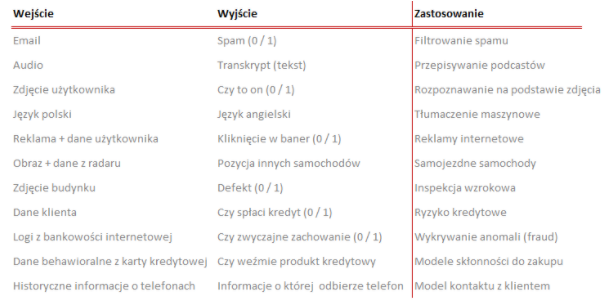
\includegraphics[width=0.9\linewidth]{S1_1.png}
	\caption{Przykładowe zastosowania uczenia nadzorowanego}
\end{figure}

\textbf{Przykłady zastosowania:} zarządzanie ryzykiem; wykrywanie nadużyć; personalizacja interakcji; rozpoznawanie mowy, tekstu i obrazu oraz segmentacji klientów.\\


\centerline{\textbf{Uczenie nienadzorowane}}

Uczenie się bez nadzoru jest bardzo przydatne w \textbf{analizie eksploracyjnej} (\textit{exploratory analysis}), ponieważ potrafi automatycznie identyfikować strukturę danych. Na przykład, jeśli analityk próbuje segmentować konsumentów, wyniki uczenia bez nadzoru mogą być doskonałym punktem wyjścia do ich analizy. W sytuacjach, w których zaproponowanie trendów w danych jest niemożliwe lub niepraktyczne, uczenie się bez nadzoru może zapewnić wstępne spostrzeżenia, które można następnie wykorzystać do przetestowania poszczególnych hipotez. \\

\textbf{Redukcja wymiarów} (możliwa do uzyskania dzięki metodom nienadzorowanym) odnosi się do metod używanych do reprezentowania danych przy użyciu mniejszej liczby kolumn lub funkcji. Podczas uczenia się reprezentacji chcemy poznać relacje między poszczególnymi funkcjami, umożliwiając nam reprezentowanie naszych danych przy użyciu postaci reprezentacji, łączącej początkowe cechy. Ta „ukryta struktura” jest często reprezentowana przy użyciu znacznie mniejszej liczby funkcji niż początkowo, więc może sprawić, że dalsze przetwarzanie danych będzie o wiele mniej intensywne, i może wyeliminować zbędne funkcje.

\textbf{Przykłady zastosowania:} analiza koszyka zakupowego, wykrywanie anomalii, rozpoznawanie podobnych obiektów.
